% Section content template for individual Educative lessons
% This file contains the actual content for a specific section
% Generated from Educative API section content

% Section: Design of a Payment System
% Section ID: 4751598016135168
% Section Slug: design-of-a-payment-system
% Generated: 2025-12-08T15:31:47.240717

In the previous lesson, we explored the working of the payment system, defined key requirements, and estimated different resources. Now , let's expand our discussion by starting with the high-level design of the payment system.

\subsection{High-level design}\label{uCksyrjwiRpXQy4HANZl4}
\\
Let's understand the high-level design of the payment system with the following illustration:

\begin{figure}[htbp]
 \centering
 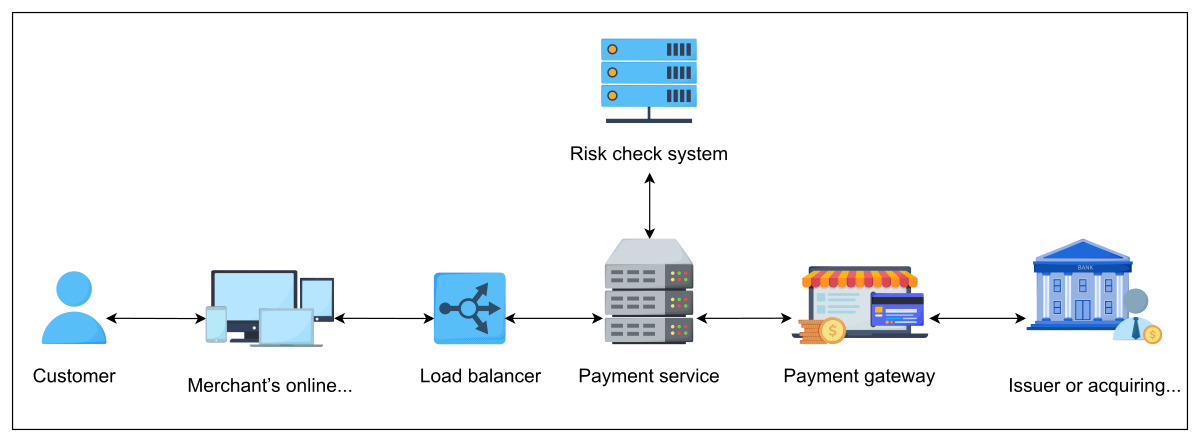
\includegraphics[width=0.5\textwidth]{Images/chapter_40/section_4751598016135168/5621166490124288.png}
 \caption{High-level design of the payment system}
\end{figure}

\begin{enumerate}
\item
\protect\phantomsection\label{xyTQICFRfD0rGcrgfJPxP}
When a customer pushes the payment button on the merchant's online store, an event is generated, which triggers the payment service.
\item
\protect\phantomsection\label{bvBAeziOj3F-Rbdk5QyLY}
The payment service processes the customer's necessary information and sends the transaction details to the risk check system for fraud detection and risk assessment.
\item
\protect\phantomsection\label{Q1-GEvuCjUt9lY83ms6B7}
If the transaction passes the risk checks, the payment service forwards the request to the payment gateway.
\item
\protect\phantomsection\label{5unDgF8hHICrgMCqlmcNu}
The payment gateway verifies the payment details and checks for correctness. Once validated, the request is forwarded to the issuer's bank.
\item
\protect\phantomsection\label{zLbd6DOw9vbh2YPCaDO7B}
The issuer bank processes the request and sends the required payment to the payment service, which deposits it into the merchant's account.
\item
\protect\phantomsection\label{gx8xQbPEPNnuLgEUEftTR}
The merchant's account is updated to reflect the credited amount on successful transactions.
\end{enumerate}
\\
How does decoupling fraud checks from the payment gateway improve scalability and security?
\\
Use the AI assessment widget below to submit your solution and get an interactive response.

\textbf{Question:}

Decoupling fraud checks

\textbf{Reference Answer:}

Decoupling fraud checks keeps the gateway lightweight while a separate fraud service performs advanced risk analysis. It improves scalability by allowing each system to scale independently, enhances security by reducing the gateway's attack surface, and increases resilience because fraud failures won't halt payment processing.

We have explored the payment system's high-level design. Before moving to the detailed design, let's discuss some essential APIs, which define users' entry points to the system:

\subsection{API design}\label{_jNkIX5lj4BO1BnLMgeMD}
\\
The following are the essential APIs that meet our functional requirements.

\subsubsection{User registration and authentication}\label{iZ6VydMlG0oHFhzpIzzhu}
\\
The user registration and authentication consist of the following two APIs.

\begin{itemize}
\item
\protect\phantomsection\label{LZzn0e6JRUg7zSYcfhcvR}
\textbf{User registration:} We have the following API for user registration.
\end{itemize}

\begin{lstlisting}[language=plaintext]
registerUser(username, email, password)
\end{lstlisting}

Under the hood, the \texttt{registerUser} API protects the password by hashing it before saving it to the database. The parameters in the API call are explained in the following table:

\begin{table}[htbp]
\centering
\small
\adjustbox{max width=\textwidth}{
\begin{tabular}{|p{0.316\textwidth}|p{0.634\textwidth}|}
\hline
\textbf{Parameter} & \textbf{Description} \\
\hline
\texttt{username} & A unique user name opted for by the customer. \\
\hline
\texttt{email} & Customer's email id to be used later in the authentication phase. \\
\hline
\texttt{password} & The customer's password is used for authentication later. \\
\hline
\end{tabular}
}
\end{table}

\begin{itemize}
\item
\protect\phantomsection\label{lfkGNFzeOlJGdVMKSK0co}
\textbf{User authentication:} To authenticate users, we use the following API, which we assume is the basic authentication mechanism.
\end{itemize}

\begin{lstlisting}[language=plaintext]
authenticateUser(username, password)
\end{lstlisting}

\subsubsection{Payment processing}\label{hlEdLx_mAmGR_mX544Zu6}
\\
In payment processing, we have the following APIs, which perform different task's including the following:

\begin{itemize}
\item
\protect\phantomsection\label{awt_lJ-8QOin-24CI4VMy}
\textbf{Payment authorization:} This API requests authorization for a payment transaction. It verifies whether the customer has sufficient funds or credit to cover the transaction amount and associates the transaction with the intended merchant. Upon successful verification, it returns an authorization code for the specified payment details.
\end{itemize}

\begin{lstlisting}[language=plaintext]
authorizePayment(amount, card_number, expiration_date, CVV, merchant_id)
\end{lstlisting}

Let's describe the parameters in the following table:

\begin{table}[htbp]
\centering
\small
\adjustbox{max width=\textwidth}{
\begin{tabular}{|p{0.316\textwidth}|p{0.634\textwidth}|}
\hline
\textbf{Parameter} & \textbf{Description} \\
\hline
\texttt{amount} & The amount to be paid by the customer for a purchase. \\
\hline
\texttt{card\_number} & 16-digit customer's payment card number. \\
\hline
\texttt{expiration\_date} & The expiry date of the payment card. \\
\hline
\texttt{CVV} & A 3-digit card verification value of the payment card. \\
\hline
\texttt{merchant\_id} & A unique identifier for the merchant receiving the payment. Used to route the transaction and reserve funds for the correct merchant account. \\
\hline
\end{tabular}
}
\end{table}

\begin{itemize}
\item
\protect\phantomsection\label{j-RuuWPXWcB1Ielal3eBV}
\textbf{Payment capture:} This API enables us to capture authorized funds after successful payment authorization, complete the transaction, and transfer the funds to the merchant's account.
\end{itemize}

\begin{lstlisting}[language=plaintext]
capturePayment(authorization_code, amount)
\end{lstlisting}

\begin{table}[htbp]
\centering
\small
\adjustbox{max width=\textwidth}{
\begin{tabular}{|p{0.316\textwidth}|p{0.634\textwidth}|}
\hline
\textbf{Parameter} & \textbf{Description} \\
\hline
\hfill\break {\texttt{}}\texttt{authorization\_code} & The authorization code provided by the \texttt{authorizePayment} API upon successful verification. \\
\hline
\texttt{amount} & The amount to be deducted from the customer's account and transferred to the merchant's account. \\
\hline
\end{tabular}
}
\end{table}

\begin{itemize}
\item
\protect\phantomsection\label{A9GZiDJ1g8xJJvUPNuSQd}
\textbf{Verify payment status:} This API checks the status of a payment transaction, allowing us to confirm whether a payment was successful or declined.
\end{itemize}

\begin{lstlisting}[language=plaintext]
checkPaymentStatus(transaction_id)
\end{lstlisting}

\begin{itemize}
\item
\protect\phantomsection\label{5uRkQaLbO6VxJvldxnMz6}
\textbf{Transaction history:} This API returns a customer's transaction history during the specified date range.
\end{itemize}

\begin{lstlisting}[language=plaintext]
getTransactionHistory(customer_id, start_date, end_date)
\end{lstlisting}

\begin{table}[htbp]
\centering
\small
\adjustbox{max width=\textwidth}{
\begin{tabular}{|p{0.316\textwidth}|p{0.634\textwidth}|}
\hline
\textbf{Parameter} & \textbf{Description} \\
\hline
\texttt{customer\_id} & The customer's ID is the one who has requested transaction history. \\
\hline
\texttt{start\_date} & The start date of the transaction is to be displayed to a customer. \\
\hline
\texttt{end\_date} & The end date of the transaction to be displayed to a customer. \\
\hline
\end{tabular}
}
\end{table}

We have explored the payment system's API design. Now, let's examine the storage schema that supports these APIs in the following section:

\subsection{Storage schema}\label{fKg8ONvDNsWwYwuOICUD0}
\\
Each of the above APIs requires support from the database. Let's understand how the payment system stores different types of information:

\begin{figure}[htbp]
 \centering
 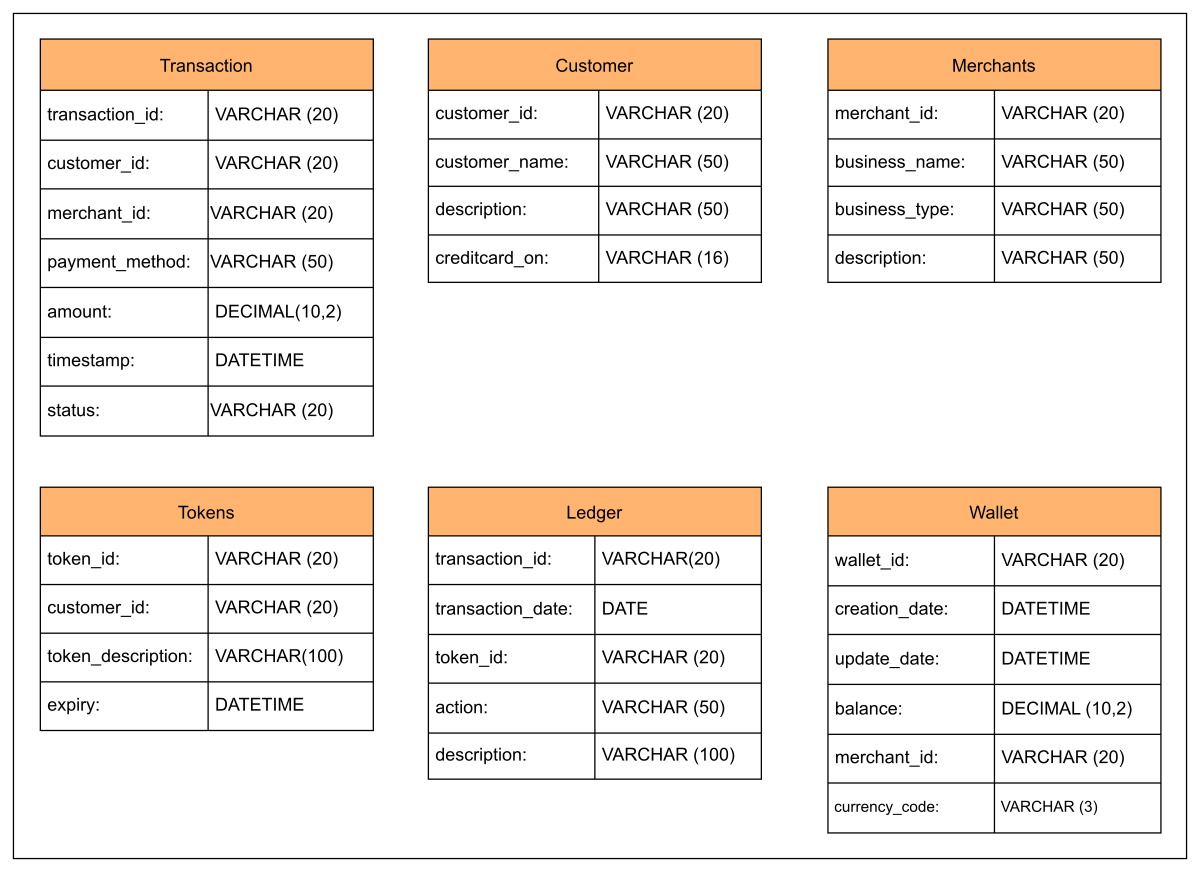
\includegraphics[width=0.5\textwidth]{Images/chapter_40/section_4751598016135168/6098452179976192.png}
 \caption{Payment system storage schema overview}
\end{figure}

We have explored the payment system's storage schema. Now, let's move to its detailed design in the following section:

\subsection{Detailed design}\label{c8EC8XbknQtYeRltJhFW4}
\\
Let's examine the detailed design of the payment system. The illustration below highlights the various components involved in the system:

\begin{figure}[htbp]
 \centering
 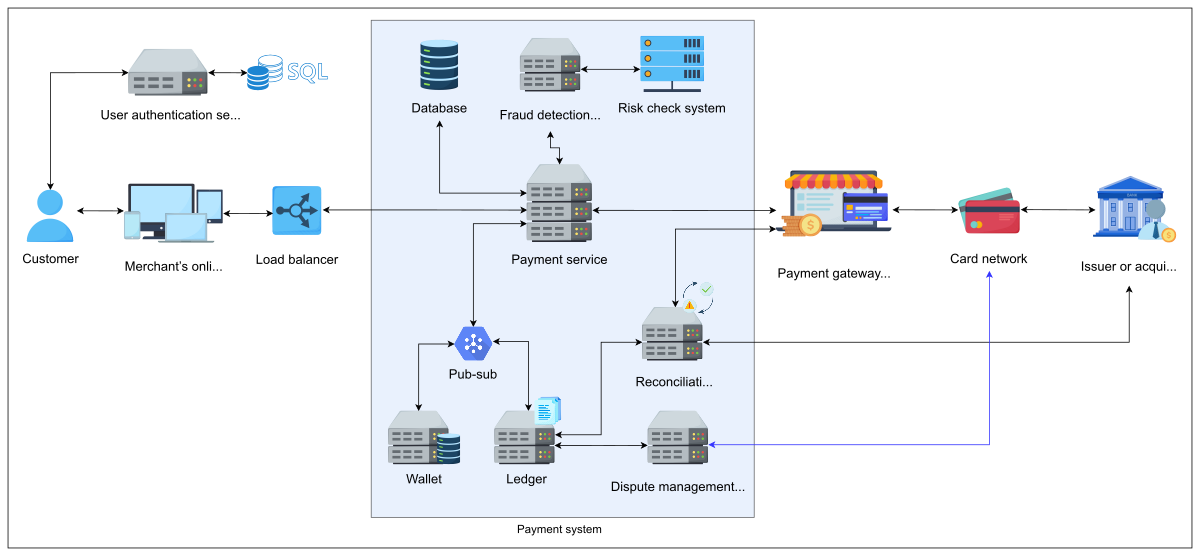
\includegraphics[width=0.5\textwidth]{Images/chapter_40/section_4751598016135168/6365908148551680.png}
 \caption{Detailed design of the payment system}
\end{figure}

Initially, a customer selects a product or service via the merchant's online store and proceeds to the checkout page, where they provide their payment detail. The payment details include the card number, cardholder name, CVV or CVC(The Card Verification Value (CVV) or Card Verification Code (CVC) is a three- or four-digit security code located on the back of most credit and debit cards.), and expiration date. Before initiating the payment, the customer is authenticated via the~user authentication service, which verifies their identity against stored credentials in the~SQL database. Once authenticated, and upon clicking the ``pay'' (or ``buy'') button, an event is generated that hits the~payment service~for processing the provided information.
\\
Let's understand the working of each component in the payment System Design to have a clear understanding of the system:

\begin{itemize}
\item
\protect\phantomsection\label{p2jCH1YPRpg0Op-dvmxdS}
\textbf{Payment service:} The payment service receives and stores the customer-generated payment event in the associated databases. It also performs initial security operations to verify that the request contains no malicious actors or is susceptible to fraudulent activity. It then sends the payment details to the fraud detection service.
\item
\protect\phantomsection\label{pA8PR31tmunNqAM4l95Ei}
\textbf{Fraud detection service:}~This service identifies and mitigates fraudulent transactions in real time. It analyzes transaction patterns, flags suspicious activities, and works with the risk check system to block high-risk payments while ensuring that legitimate transactions are not mistakenly flagged as fraudulent. Transactions flagged as suspicious may be rejected or require additional authentication.
\item
\protect\phantomsection\label{bnqhxmrmXLvjEvU1fqLPP}
\textbf{Risk check system:} The risk check system works alongside the fraud detection service to assess each transaction's risk level. It evaluates multiple factors, including device fingerprinting, transaction history, location-based risk analysis, and velocity checks. Based on the analysis, it assigns a risk score to the transaction and determines whether to proceed, challenge, or block the payment.
\end{itemize}

\begin{quote}
\textbf{Quiz:}
\textbf{Question 1:} If a fraud detection system is already in place, what additional value does a dedicated risk check system provide?
\textbf{Answer:} While a fraud detection system focuses primarily on identifying and preventing malicious or unauthorized activities, a risk check system serves a broader purpose by evaluating the overall risk profile of a transaction or user, even when no fraud is detected. This layered approach helps mitigate not only fraud but also financial, operational,

and reputational risks, offering a more comprehensive defense strategy.
\end{quote}

\begin{itemize}
\item
\protect\phantomsection\label{aFYVsvLKG52BRryCfKfTd}
\textbf{Payment gateway (payment service provider):} The payment gateway performs extensive security checks on the request. Due to its complexity, a third party often performs the risk check, a specialized process. The payment gateway is primarily responsible for moving money from the customer's account to the merchant's. Since the payment gateway also acts as a PSP, it offers some secondary services, such as maintaining sessions during the payment process, handling different requests, such as refunds, generating invoices, etc.
\item
\protect\phantomsection\label{va2hniZq7fUnaPcMuFsGN}
\textbf{Card networks:} Since customers normally pay via their credit or debit cards, there should be a mechanism to verify card information. This verification is carried out via the card network. The interaction between a payment gateway and the card network takes place via the APIs provided by the card network.
\item
\protect\phantomsection\label{3pD1Vg0MEOIVW3TDdoDOA}
\textbf{Wallet:}~When the payment gateway successfully processes the payment, the~payment service~(acting as the coordinator) updates the merchant's wallet in the database to reflect the new balance. This wallet is used to track the merchant's total revenue. Sometimes, multiple orders from different sellers might occur in a single purchase. The payment service processes each such order separately. Each seller's wallet is updated after receiving the buyer's account payment.
\item
\protect\phantomsection\label{ezxBOkiUi2j_Lq7ryRvLJ}
\textbf{Ledger:} When the payment service updates the wallet, the ledger service appends a new immutable entry to the ledger database. This entry typically includes the transaction ID, amount, currency, involved parties, transaction type (payment or refund), timestamp, and status. These records provide a reliable and auditable trail of all financial operations.
\end{itemize}

\begin{quote}
\textbf{Quiz:}
\textbf{Question 1:} Where are the customer\textquotesingle s payment details encrypted during a purchase?
\textbf{Answer:} Customer's payment details in the system are encrypted at several key points: 1. Client-side encryption: Payment details are encrypted on the customer\textquotesingle s device (e.g., computer or smartphone)

before being transmitted over the internet. 2. During data transmission: Encrypted connections (SSL/TLS) secure the transmission of payment details between the customer and the payment system's servers. 3. Payment gateway: The payment gateway also encrypts payment details to facilitate customer and merchant transactions. 4.

Storage encryption: Payment details may be temporarily stored and should be encrypted at rest for security. For example, when the payment service receives a payment event, it stores the event details in the database after applying the necessary encryption. Encryption is a vital security measure, complemented by access controls and compliance with industry standards like  PCI DSS: PCI DSS stands for Payment Card Industry Data Security Standard. It is a set of security standards and requirements designed to ensure the secure handling of credit and debit card information during payment transactions. , to safeguard customer payment information.
\end{quote}

\begin{itemize}
\item
\protect\phantomsection\label{kpXGDPsWYQBGbvwvo6LMy}
\textbf{Reconciliation system:} Reconciliation in the payment system is the process of matching and verifying financial records to ensure that all transactions are accurately accounted for and that there are no discrepancies between different records and statements. It is a critical financial management component that allows the ledgers to align with the payment gateway (or PSP) transaction records. Reconciliation is particularly important in payment systems because it helps identify and resolve errors, fraud, and discrepancies.\\
Periodically, the PSPs send the settlement file to the clients at the day's end. The settlement file includes the balance of the account and all the transactions that occurred on that account during the day. The reconciliation system analyzes the settlement file and reconciles the information in the settlement file with the information in the ledger system. It also helps us to verify that the payment system is consistent internally.\\
For example, if a merchant received three payments during the day---one for \$50, another for \$100, and a third for \$75---the settlement file from the PSP would list these transactions and a total settlement amount of \$225. The reconciliation system cross-checks this file against the internal ledger entries for the same merchant. The data is reconciled if all three transactions exist in the ledger with matching amounts and timestamps. If there's a mismatch, the system flags it for further investigation.
\end{itemize}

\begin{quote}
\textbf{Quiz:}
\textbf{Question 1:} What happens if a mismatch is found during reconciliation?
\textbf{Answer:} If a mismatch is found, the reconciliation system alerts and logs the discrepancy for further investigation, the issue could be missing transactions, duplicate entries, timing delays, or data corruption. The system may: - Temporarily hold settlements until the mismatch is resolved. - Trigger a reprocessing of affected transactions. - Notify the operations team or initiate automated correction workflows,

depending on the severity.
\end{quote}

\begin{itemize}
\item
\protect\phantomsection\label{7yrmjexnxu3fPOnN9Aliz}
\textbf{Dispute management service:}~This service handles transaction disputes between customers, merchants, and financial institutions. It collects transaction details, collaborates with the issuer bank and card network, and processes chargebacks if necessary. It upholds compliance with financial regulations and maintains dispute records to prevent fraudulent claims.
\end{itemize}
\\
We have discussed the detailed design, but a few questions could arise while designing a payment system. For example:

\begin{enumerate}
\item
\protect\phantomsection\label{ZDr732zzNemHfjRuf6-Wa}
How should we guarantee transaction completion?
\item
\protect\phantomsection\label{F-A5fWMmUkP5aq_jIalGS}
How can we handle transient failures, and what strategies should we adopt?
\item
\protect\phantomsection\label{7cLQlK6yNYRGguojAUbFw}
How can we avoid persistent failures?
\end{enumerate}
\\
Let's address the above questions one by one:

\subsection{Transaction completion}\label{K9hcJg_zUMlZT2Fi1ssZq}
\\
Within the payment system, multiple interconnected services collaborate to execute a transaction. The primary concern is ensuring that requests aren't lost over the network. Another possibility is that messages reach the backend system but encounter unavailable services.

\begin{figure}[htbp]
 \centering
 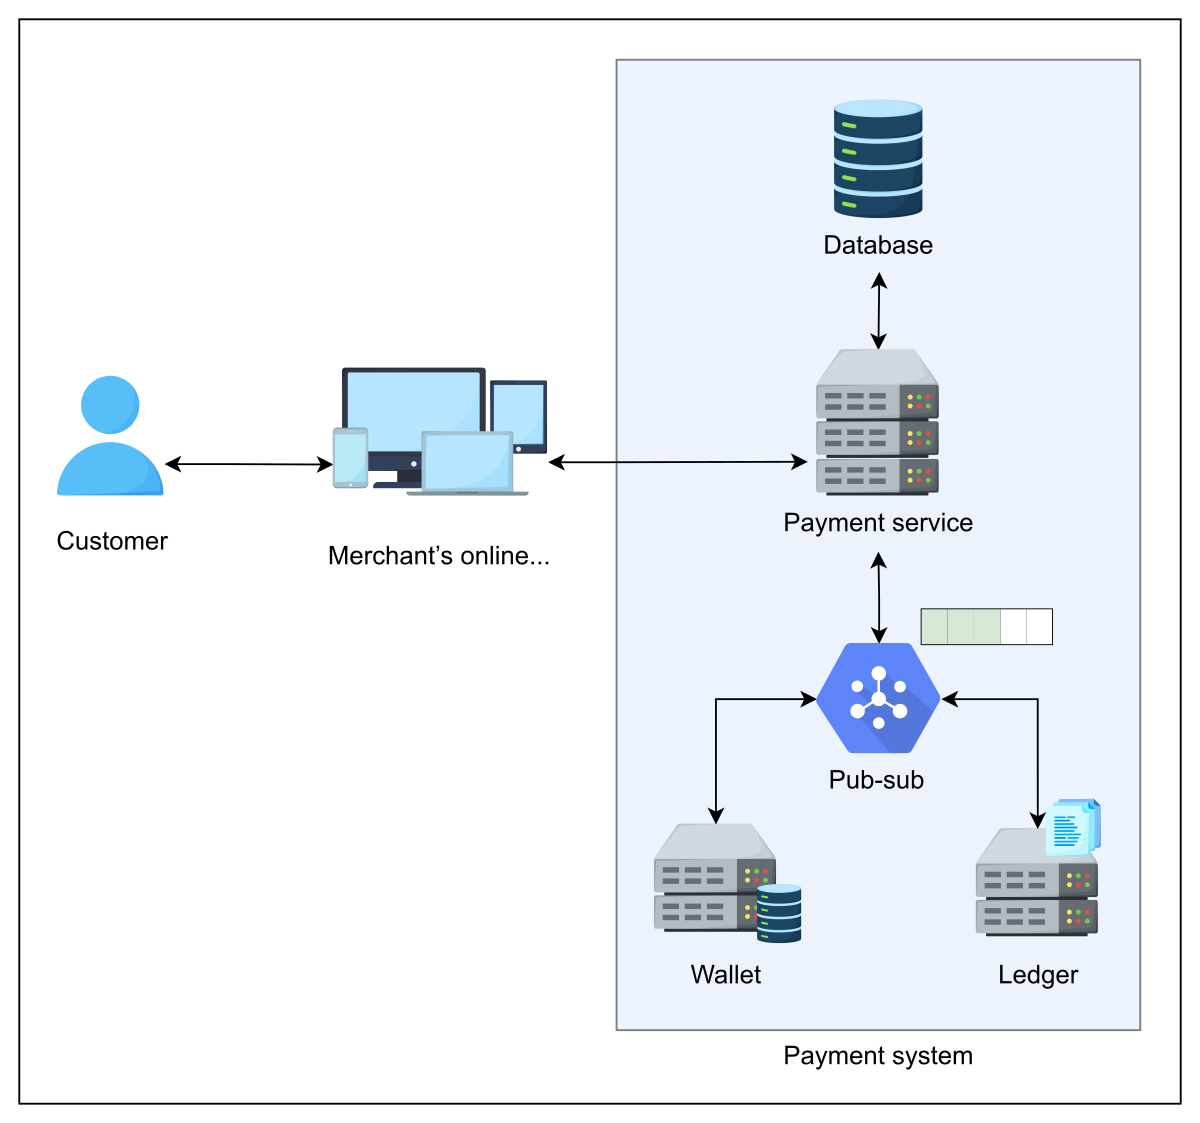
\includegraphics[width=0.5\textwidth]{Images/chapter_40/section_4751598016135168/5302298957709312.png}
 \caption{Flow of services involved in transaction completion}
\end{figure}

\hfill\break
We employ a pub-sub system like Apache Kafka to secure the completion of transactions. For each order placement or payment, we generate an event within Kafka. This approach aids in managing communication messages to prevent them from being lost in unexpected situations. While it's worth noting that Kafka itself may encounter issues, its current role is relatively straightforward, making its priority notably higher than other business-critical services. The services associated with Kafka consume these messages. A message is marked as consumed only when successfully processed, and its outcome is stored in the wallet's database and ledger.

\subsection{Transient failures}\label{8YsdYDyn2KoLeDk8G1A56}
\\
A \textbf{transient failure} refers to a temporary or short-lived problem or error that occurs in a system or process but does not indicate a permanent issue. Transient failures are typically brief and can be caused by various factors, including network glitches, temporary resource constraints, software bugs, or external factors beyond the system's control. In the payment system, it is important to avoid such temporary issues, and there needs to be a proper mechanism for resolution. To address transient failures, systems often rely on strategies such as:

\begin{itemize}
\item
\protect\phantomsection\label{IDScBaIY2Y6JTjWjq4X0w}
Retry strategy
\item
\protect\phantomsection\label{DW2A0aKUlU9dkYHj2WswH}
Timeout
\item
\protect\phantomsection\label{v4VXvarR3d-NfrTzVv2xT}
Fallback mechanism
\end{itemize}
\\
Let's examine how each of these strategies helps improve resilience in the payment system.

\subsubsection{Retry strategy}\label{o3Qz4Ul-Fim8_cdIBNh9C}
\\
The retry strategy helps us avoid temporary network problems and ensure that the payment transactions are processed reliably. For this, we implement exponential backoff(If a payment transaction initially fails due to a temporary network problem, the system waits for a short period before attempting to retry. If the retry also fails, the system waits longer before the next attempt.) and set retry limits. The retry limits set a maximum limit on the number of retry attempts for a transaction. After reaching this limit, the request will be marked as failed and can be retried after a specific time interval.

\subsubsection{Timeout}\label{IidYNTVrOrDdr09leDapB}
\\
The purpose of implementing a timeout is to prevent waiting indefinitely for a response. When the response time becomes excessively long, the operation is terminated, and the request is marked unsuccessful. This mechanism is employed in almost every application to prevent requests from becoming stuck indefinitely. Nonetheless , handling timeouts can be a complex task. Consider a scenario in an online store where a payment request fails for an order. The customer may observe that the purchase order wasn't processed, but various outcomes could occur in the backend, as given below:

\begin{enumerate}
\item
\protect\phantomsection\label{UDRxcv0qrlCz21j0Ghdp5}
It's possible that the payment request was effectively initiated, but the response from the payment service might have been lost in transit from the backend.
\end{enumerate}

\begin{figure}[htbp]
 \centering
 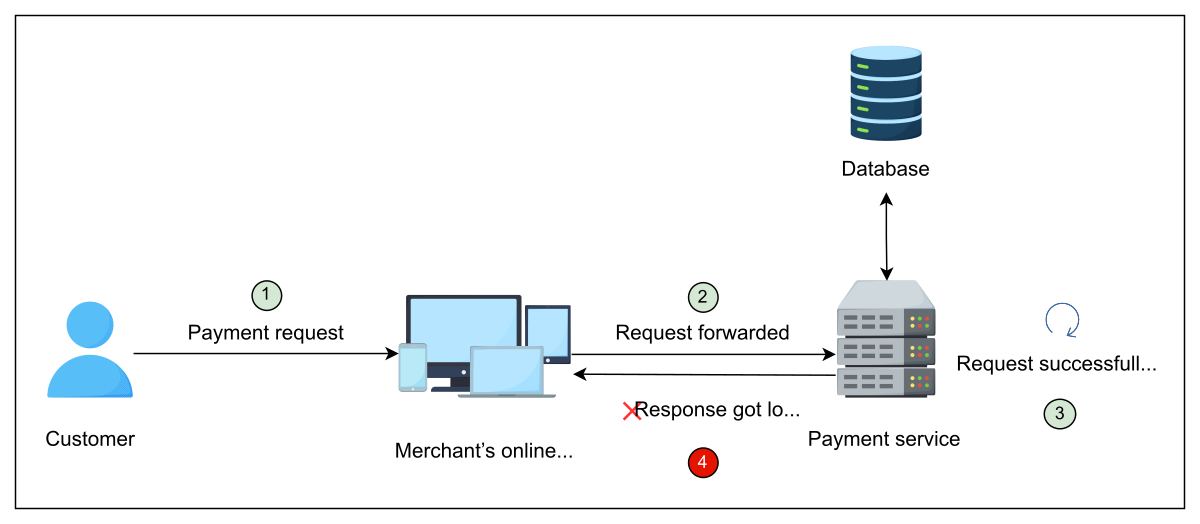
\includegraphics[width=0.5\textwidth]{Images/chapter_40/section_4751598016135168/5632244217413632.png}
 \caption{Response from the payment service got lost in transit}
\end{figure}

\begin{enumerate}
\setcounter{enumi}{1}
\item
\protect\phantomsection\label{8WGv31SOzaRuciQDz8Opj}
The request is being processed within the payment system and has reached a point where a request timeout has occurred.
\end{enumerate}

\begin{figure}[htbp]
 \centering
 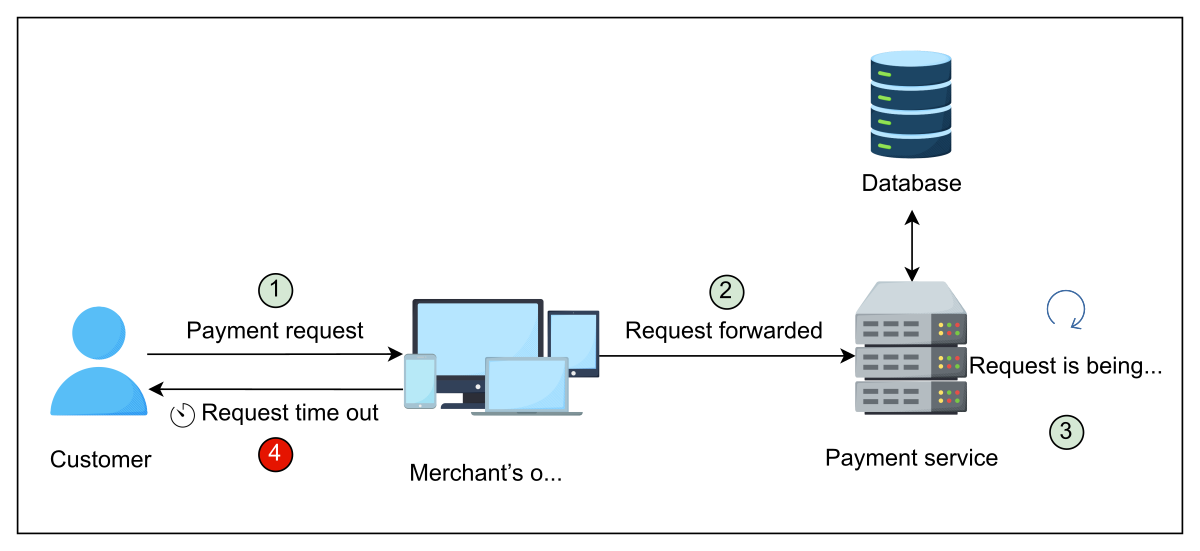
\includegraphics[width=0.5\textwidth]{Images/chapter_40/section_4751598016135168/4563682795061248.png}
 \caption{Request time out}
\end{figure}

\begin{enumerate}
\setcounter{enumi}{2}
\item
\protect\phantomsection\label{JbIpIBgpVnwxqIVrx29-g}
The third scenario could be that the request is lost during transit and has not reached the payment service.
\end{enumerate}

\begin{figure}[htbp]
 \centering
 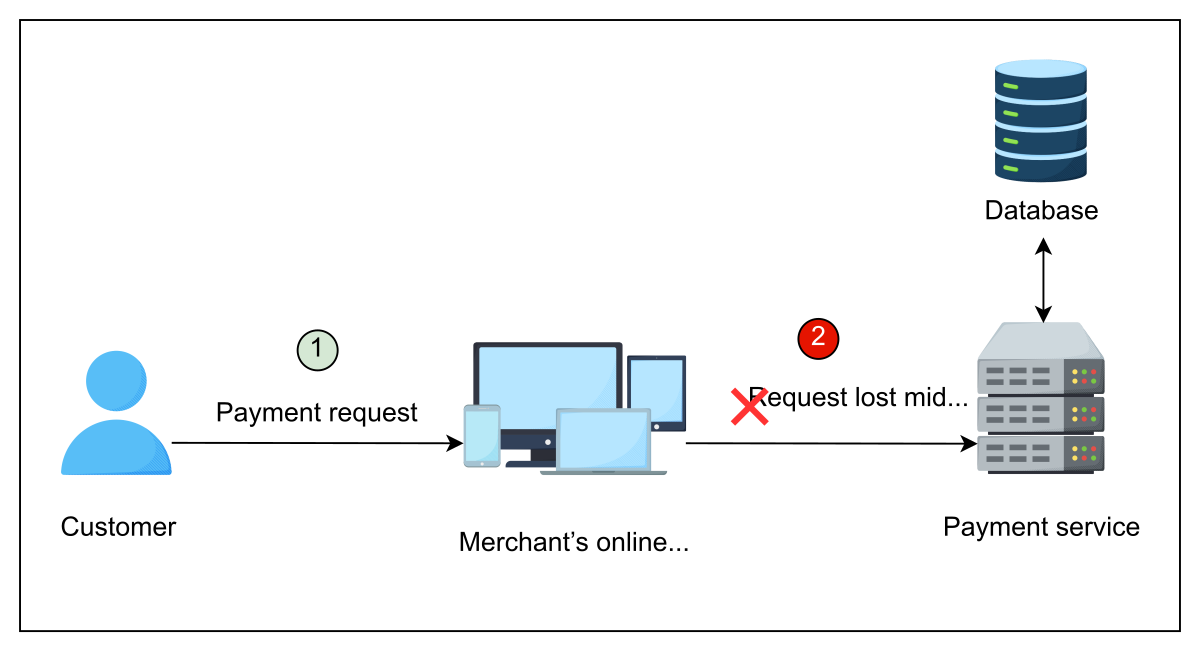
\includegraphics[width=0.5\textwidth]{Images/chapter_40/section_4751598016135168/5795770869350400.png}
 \caption{Request got lost in midway}
\end{figure}

In all the above three scenarios, what status should we give a customer? For example, if we mark the request as failed, the customer might think the order didn't succeed, but it may have succeeded, and they could get charged. However, the request was marked as failed due to a lack of response. What happens if the customer retries the operation? This is where\textbf{~idempotency}~comes into play. Idempotency ensures that even if a customer retries a request, the system will handle it in a way that prevents duplicate charges or unintended consequences.

\begin{quote}
\textbf{Quiz:}
\textbf{Question 1:} How to ensure that there are no duplicate payments when a customer hits the buy button many times for a single purchase?
\textbf{Answer:} We can create a distinct transaction identifier (like an order number or payment ID) for every transaction or purchase, which serves as our idempotence key. This key is stored in our database when the customer initiates the payment and the request's status (for example, succeeded,

failed, or in progress). If a customer accidentally clicks the ``buy'' button twice or generates a duplicate request for the same purchase,
they won't be charged, as the idempotence key in the database prevents multiple charges.
\textbf{Question 2:} How big should be the time-out value?
\textbf{Answer:} Deciding the timeout value depends on how complex the payments are and what kind of system we use. For basic online shopping, a small value is usually fine. But we might need a larger value if we are doing something more complex, like sending money internationally or booking a flight.

It's also a good idea to follow the guidelines of the payment gateways we are using. We must balance making it easy for customers and keeping things secure. If we set the value very small, customers might get frustrated. If it's too large, it could be a security risk. As a rule of thumb, think about how long it takes for most customers to finish their payment and use that as a guide.
\end{quote}

\subsubsection{Fallback}\label{n8VZsViJtCNnubo3LUcyg}
\\
\textbf{Fallback} typically refers to a backup method or alternative process that can be used when the primary payment method or technology fails or encounters difficulties. It enables a service to continue executing even when requests to a dependent service encounter failures. As an example, during the payment process, a request might be dispatched to the fraud check service, which, in turn, may respond with an internal server error. Instead of halting the entire computation due to the absence of a response, we can substitute a fallback value(A fallback value is a predefined or default value that is used when a specific condition or scenario occurs, typically when the system encounters an unexpected situation or cannot retrieve the desired data or perform a certain operation.). For example, in the case of very small transactions, we can permit the transaction to proceed. This approach represents a balance between assuming certain risks and ensuring customer satisfaction by minimizing wait times.

\subsection{Achieving requirements}\label{8OeDcDiOn3s5jOHLsV3xh}
\\
Let's see how the proposed payment System Design satisfies both functional and non-functional requirements.

\subsubsection{Achieving functional requirements}\label{R-6i9aQCZotGVu4B7hG0f}
\\
Let's examine how the payment system fulfills the functional requirements that we outlined in the previous lesson, in the following table:

\begin{table}[htbp]
\centering
\small
\adjustbox{max width=\textwidth}{
\begin{tabular}{|p{0.324\textwidth}|p{0.626\textwidth}|}
\hline
\textbf{Functional Requirements} & \textbf{Techniques} \\
\hline
User registration and authentication & \begin{itemize} \tightlist \item Handled by the merchant\textquotesingle s online store. It provides secure login, session management, and user identity validation \item Authenticated requests forwarded to the payment service \end{itemize} \\
\hline
Payment processing & \begin{itemize} \tightlist \item Payment processing is handled by the payment service in conjunction with other coordinated services, such as PSP, fraud detection services, and reconciliation services, among others. \end{itemize} \\
\hline
Transaction history & \begin{itemize} \tightlist \item The ledger stores immutable transaction logs, including details such as ID, amount, currency, involved parties, status, and timestamp. \end{itemize} \\
\hline
Balance management & \begin{itemize} \tightlist \item The~wallet~maintains up-to-date merchant balances by reflecting successful payments and refunds. \item The~payment service~updates the wallet after each transaction.~ \item Ledger provides an auditable balance history for verification \end{itemize} \\
\hline
Mobile accessibility & \begin{itemize} \tightlist \item Enabled by a responsive~Merchant's online store~UI. \end{itemize} \\
\hline
\end{tabular}
}
\end{table}

\subsubsection{Achieving non-functional requirements}\label{RgnyKob3G8nPr7HbwiI_2}
\\
Beyond core features, a payment system must be secure, scalable, and resilient. The table below shows how our proposed design meets these essential non-functional requirements:

\begin{table}[htbp]
\centering
\small
\adjustbox{max width=\textwidth}{
\begin{tabular}{|p{0.301\textwidth}|p{0.649\textwidth}|}
\hline
\textbf{Non-functional Requirements} & \textbf{Techniques} \\
\hline
Data integrity and security & \begin{itemize} \tightlist \item Adhere to industry security standards such as PCI DSS (Payment Card Industry Data Security Standard). \item Use robust encryption and secure storage mechanisms.~ \end{itemize} \\
\hline
Reliability and availability & \begin{itemize} \tightlist \item Used redundant services (payment, reconciliation, risk check) to prevent failures.~ \item Replicate data across multiple data centers for high availability.~ \item Utilize local load balancers to exclude failed servers.~ \item Deploy global load balancers to redirect traffic during regional failures. \end{itemize} \\
\hline
Scalability & \begin{itemize} \tightlist \item Scale databases efficiently and cache frequently accessed data to optimize performance.~ \item Implement load balancing to prevent bottlenecks.~ \item Enable monitoring and automated scaling for dynamic resource allocation. \end{itemize} \\
\hline
Performance & \begin{itemize} \tightlist \item Process transactions asynchronously to decouple services.~ \item Ensure sufficient bandwidth during peak times.~ \item Implement transient failure strategies (retry, timeout, and fallback) to ensure timely responses. \end{itemize} \\
\hline
\end{tabular}
}
\end{table}

\subsection{Conclusion}\label{SfvIAwjza6302gP02GWjL}
\\
Designing a secure and resilient payment system requires a balance between efficiency, reliability, and fraud prevention. In this chapter, we've explored the entire payment process, from transaction authorization to settlement, while addressing the functional and non-functional requirements that shape such a system. Our proposed design focuses on enabling payments through credit and debit cards. While the desigOur proposed design focuses on enabling payments through credit and debit cards. While the design addresses key components, it's essential to note that certain entities, such as banks, online merchant stores, and risk-check services, are part of larger systems that fall outside the scope of this specific design problem.\\
A well architected payment system ensures seamless, secure transactions while minimizing risks and maintaining financial integrity. By thoughtfully selecting system components and architectural patterns, businesses can build scalable, robust, and trustworthy payment infrastructures that meet current industry demands and are adaptable to future challenges.

% End of section content